\documentclass[a4paper,11pt]{article}
\usepackage[T1]{fontenc}
\usepackage[utf8]{inputenc}
\usepackage{lmodern}
\usepackage{amsmath}
\usepackage{amsfonts}
\usepackage{amssymb}
\usepackage{amsthm}
\usepackage{graphicx}
\usepackage{color}
\usepackage{url}
\usepackage{textcomp}
\DeclareMathOperator*{\argmax}{argmax}
\DeclareMathOperator*{\argmin}{argmin}

\title{Value Iteration}
\author{Joshua Tsang}
\date{\today}

\begin{document}

\maketitle
\tableofcontents

\section{Foundational Concepts}

It is instructive intially discuss the foundational concepts in Markov Decision Problems (MDP) and Reinforcement Learning (RL).  Consider the problem shown in Figure \ref{fig:1d-grid-world-problem-statement} where an agent is located in one of the grid positions.

\begin{figure}
    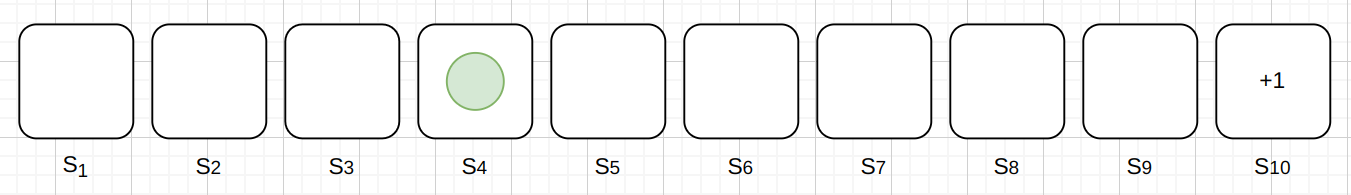
\includegraphics[width=\textwidth]{images/1d-grid-world-problem-statement.png}
    \caption{1D Grid World MDP with an assigned reward of $+10$ in state $s_{10}$, termed the terminal state.  The agent currently sits in state $s_4$ and the goal of the problem is for the agent to take actions to maximise its reward.  At each state other than the terminal state, there is a negative reward of $-1$.  Drawn with draw.io and saved in Google Drive as 1D\_grid\_world.drawio.}
    \label{fig:1d-grid-world-problem-statement}
\end{figure}


\begin{itemize}
    \item State Space and State: The finite State Space of a system is denoted $S$ where a state $s$ denotes a certain configuration of the system i.e. $s \in S$.  For example, in Figure \ref{fig:1d-grid-world-problem-statement} the agent is currently in state $s_4$, with the neighbouring states, $\{s'\}$, being $s_3$ and $s_5$.
    \item Actions: For each state, $s_i$, that the system resides in a set of available actions, $\{a_k\}$, can be taken that transition the system to another state, $s_j$.  For Figure \ref{fig:1d-grid-world-problem-statement} the available actions at state $s_4$ are \verb|(move left)| and \verb|(move right)|.  One could think of a graph where nodes are states and the edges are actions.
    \item Policy: A policy, denoted $\pi$, dictates the action to take for a given state.  It is often written as a function $\pi(s, a)$ where it is formally defined as:
    \begin{equation} \label{eqn:policy_formal_definition}
        \pi(s,a) = P(A_t=a|S_t=s)
    \end{equation}
    which is the probability of taking action $a$ given the system is in state $s$ at time step $t$. The goal of RL is to learn the optimal policy $\pi(s,a)$ to maximise future rewards/returns (explained next). As a foreshadow, policy functions are often expressed as an $\argmax_a$ as follows:
    \begin{equation} \label{eqn:value_iteration_foreshadow}
        \pi(s,a) = \argmax_a \sum_{s'} P(s',r|s,a)[r + \gamma v_{\pi}(s')]
    \end{equation}
    i.e. the policy function returns the action $a$ that transitions the agent to the neighbouring state $s'$ that yields the maximum transition-probability-weighted sum of the returns.
    \item Reward: Numerical reward can be associated with certain states and actions, represented as $R_t$ for the current time step.  In the case of Figure \ref{fig:1d-grid-world-problem-statement}, there is a fixed reward of $+10$ at state $s_{10}$ and the other states have a reward of $-1$.  The goal of RL can be considered to be finding the sequence of actions that maximise the sum of rewards to achieve a sucessful episode i.e. the agent reaches the terminal state $s_{10}$.
    \item Episodes:  MDPs have the characteristic of being finite i.e. they end within a finite number of time steps, denoted $T$.  More specifically, an episode is a sequence of states, actions and rewards that start at some state and end in the terminal state.
    \item Return or "Future Gains":  Usually denoted $G_t$ it is the sum of rewards gained by the agent {\it after} time step $t$, define as:
    \begin{equation} \label{eqn:return_G_t}
        G_t = R_{t+1} + R_{t+2} + ... + R_{T}
    \end{equation}
    Before going further, it's worth appreciating how important this concept is to the definition of state value functions, $v(s)$, which try to capture the expected rewards to be gained by being in that state, $s$.

    It is possible to introduce a discount rate $\gamma \in [0,1]$ that diminishes the rewards gained further in the future:
    \begin{equation} \label{eqn:return_G_t_discounted}
    \begin{split}
        G_t &= R_{t+1} + \gamma R_{t+2} + \gamma^2 R_{t+3} + ... + \gamma^{T-1-t} R_{T} \\
        &= \sum_{k=t+1}^{T} \gamma^{k-1-t}R_k
    \end{split}
    \end{equation}
    note how the power of $\gamma$ in the final term is $T-1-t$ and {\it not} $T$, a little thought makes this clear (for example, try write down $G_4$ where $T=8$).  Finally, we note that the discounted expression can be rewritten into a recursive expression somewhat similar to Bellman's equation:
    \begin{equation} \label{eqn:return_G_t_like_bellmans_eqn}
    \begin{split}
        G_t &= R_{t+1} + \gamma R_{t+2} + \gamma^2 R_{t+3} + ... + \gamma^{T-1-t} R_{T} \\
        &= R_{t+1} + \gamma( R_{t+2} + \gamma R_{t+3} + ... + \gamma^{T-t} R_{T}) \\
        &= R_{t+1} + \gamma G_{t+1}
    \end{split}
    \end{equation}
    Expression (\ref{eqn:return_G_t_like_bellmans_eqn}) links the current return, $G_t$, to the return at the next time step, $G_{t+1}$.
\end{itemize}

\section{Playing with Episodes}

Recall that epsiodes are a sequence of states, actions and rewards that end in the terminal state.  Each episode yields a return/gain at $T$, which is $G_T$.  To clarify concepts and develop some intuitive, consider a few episodes for the Grid World system in Figure \ref{fig:1d-grid-world-problem-statement}.  The actions are $a \in [\text{LEFT}, \text{RIGHT}]$

\begin{itemize}
  \item Episode Example 1:
  
  $[S_{t=1} = s_4, A_{t=1} = \text{RIGHT}, G_{t=1}=-1]$ \\
  $[S_{t=2} = s_5, A_{t=2} = \text{RIGHT}, G_{t=2}=-2]$ \\
  $[S_{t=3} = s_6, A_{t=3} = \text{RIGHT}, G_{t=3}=-3]$ \\
  $[S_{t=4} = s_7, A_{t=4} = \text{RIGHT}, G_{t=4}=-4]$ \\
  $[S_{t=5} = s_8, A_{t=5} = \text{RIGHT}, G_{t=5}=-5]$ \\
  $[S_{t=6} = s_9, A_{t=6} = \text{RIGHT}, G_{t=6}=-6]$ \\
  $[S_{t=7} = s_10, A_{t=7} = \text{RIGHT}, G_{t=7}=+4]$ \\

  Note that this episode yields $G_T = +4$.

  \item Episode Example 2:
  
  $[S_{t=1} = s_4, A_{t=1} = \text{RIGHT}, G_{t=1}=-1]$ \\
  $[S_{t=2} = s_5, A_{t=2} = \text{RIGHT}, G_{t=2}=-2]$ \\
  $[S_{t=3} = s_6, A_{t=3} = \text{RIGHT}, G_{t=3}=-3]$ \\
  $[S_{t=4} = s_7, A_{t=4} = \text{RIGHT}, G_{t=4}=-4]$ \\
  $[S_{t=5} = s_8, A_{t=5} = \text{LEFT}, G_{t=5}=-5]$ \\
  $[S_{t=6} = s_7, A_{t=6} = \text{RIGHT}, G_{t=6}=-6]$ \\
  $[S_{t=7} = s_8, A_{t=7} = \text{RIGHT}, G_{t=7}=-7]$ \\
  $[S_{t=8} = s_9, A_{t=8} = \text{RIGHT}, G_{t=8}=-8]$ \\
  $[S_{t=9} = s_10, A_{t=9} = \text{RIGHT}, G_{t=9}=+2]$ \\
  
  Note that this episode yields $G_T = +2$, it is lower than Episode Example 1 because at $t=5$ it backtracks by going LEFT which caused it to require a longer path, and thus suffer more from the $R_t = -1$ penalties for the non-terminal states.
\end{itemize}

\section{State Value Function, Bellman's Equation and the Principle of Optimality}

An important concept in RL is the state value function, $v_{\pi}(s)$, which captures the expected return from being in state $s$.  It is critical to realise that the subscript $\pi$ in $v_{\pi}(s)$ means it must be evaluated for a given policy $\pi$ since $v_{\pi}(s)$ is an expectation value (read: average) of potential returns by being in state $s$, which in turn depends on the expected return from state $s$'s neighbouring states, $s'$. Since $\pi{s,a}$ encapsulates the probability of transitioning to neighbouring states $s'$ from state $s$, and in turn the state values in those neighbouring states $v_\pi(s')$, therefore the policy $\pi{s,a}$ influences the expected returns.  In fact, it's prudent to think of the state value function as a function to link the state values of all states together.

\begin{equation} \label{eqn:bellmans_equation_part1}
\begin{split}
        v_\pi (s) &= \mathbb{E}[G_t|s] \\
        &= \sum_{a} \pi(a|s) \mathbb{E} [G_t|s,a]
\end{split}
\end{equation}

Using Equation (\ref{eqn:return_G_t_like_bellmans_eqn}) we can rewrite $\mathbb{E} [G_t|s, a]$ as:

\begin{equation} \label{eqn:bellmans_equation_part2}
\begin{split}
        \mathbb{E} [G_t|s, a] &= \mathbb{E} [R_{t+1} + \gamma G_{t+1}|s, a] \\
        &= \mathbb{E} [R_{t+1} + \gamma v_\pi(S_{t+1})|s, a] \\
        &= \sum_{s'} \sum_r P(s',r|s,a) [r + \gamma v_{\pi}(s')]
\end{split}
\end{equation}

Hence the final expression is:
\begin{equation} \label{eqn:bellmans_equation_part3}
\begin{split}
        v_\pi (s) &= \sum_{a} \pi(a|s) \sum_{s'} \sum_r P(s',r|s,a) [r + \gamma v_{\pi}(s')]
\end{split}
\end{equation}
Equation \ref{eqn:bellmans_equation_part3} allows us to calculate the expected return value for each state in the MDP, and in turn allows an optimal policy to be extracted. 

Don't be put off by the numerous probability `given' symbols like $P(A|B)$, since usually $B$ is the current state and action taken, it therefore just means `the probability of transitioning to $A$ given the agent is in state $s$ and taken action $a$'.  

Note that the probabilities $P(s',r|s,a)$ are nothing to do with the policy probabilities $\pi(s,a)$ but are transition probabilities intrinsic to the Markov process.  For instance, we could introduce a `drunken man' effect into the MDP in Figure \ref{fig:1d-grid-world-problem-statement} where there's only a 0.8 chance of the intended action yielding the intended outcome.  So in this case, if we're in state $s4$ then $P(s_5,r|s_4, a=\text{RIGHT}) = 0.8$ and $P(s_3,r|s_4, a=\text{RIGHT}) = 0.2$ i.e. there's a 0.2 chance of transitioning into the state in the opposite direction.  The goal of RL is to deduce the optimal policy taking into account these effects.





\section{The Quality Function}

The quality function is often defined as the sums in Equation (\ref{eqn:bellmans_equation_part3}):
\begin{equation} \label{eqn:quality_function_Q}
    Q(s,a) = \sum_{s'} \sum_r P(s',r|s,a) [r + \gamma v_{\pi}(s')]
\end{equation}
where $s'$ are the neighbouring states to the current state, $s$.  


\section{Value Iteration}

Value iteration allows one to assign state values to each state through repeated, iterative application of the value function, and the optimal policy is extracted at the end.  



\begin{figure}
    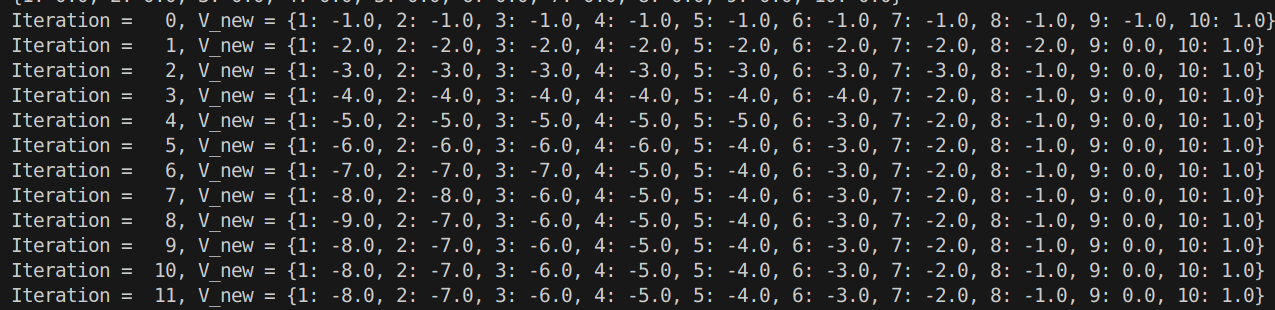
\includegraphics[width=\textwidth]{images/iters-of-value-iteration-1d-grid-world-code-output.png}
    \caption{Iterations of the value iteration algorithm.}
    \label{fig:iters-of-value-iteration-1d-grid-world-code-output}
\end{figure}


\section{Policy Iteration}

\end{document}